% Algorytmy grafowe
\section{Algorytmy grafowe}

\subsection{Algorytm Floyda-Warshalla}

\entry
Problem najlżejszych ścieżek pomiędzy wszystkimi
parami wierzchołków

\entry 
Idea:

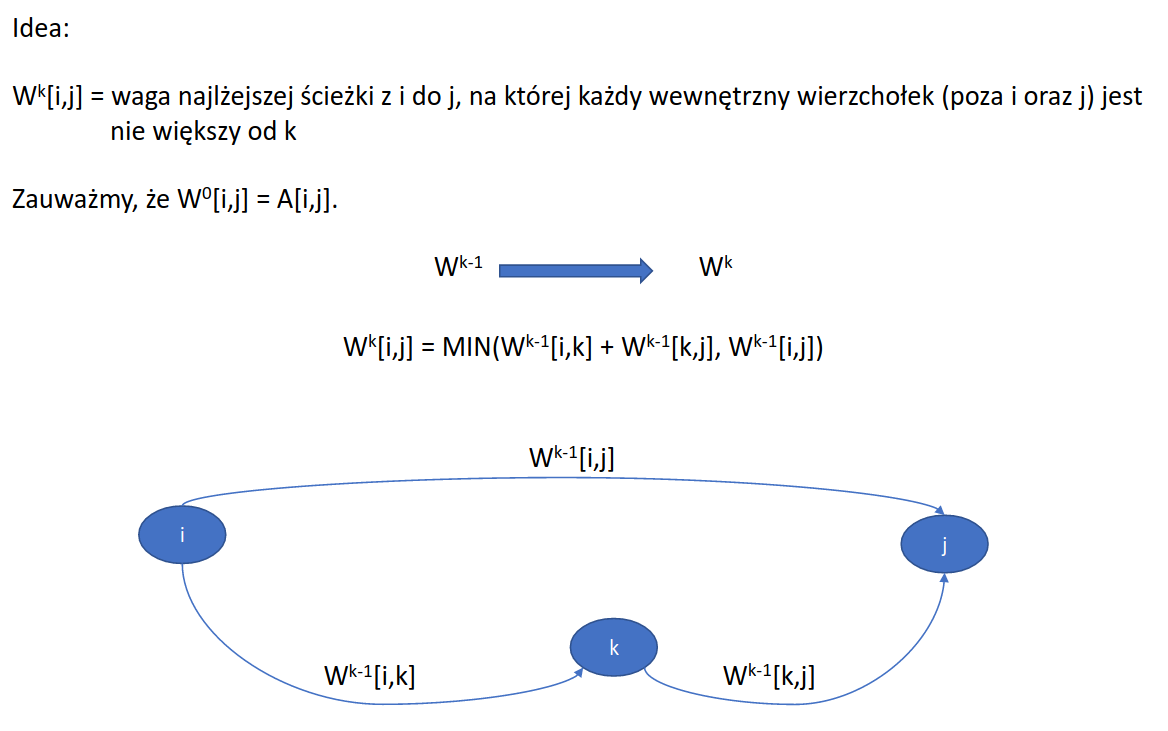
\includegraphics[scale=0.25]{ideawarszal.png}

\subsection{Spójne składowe}

\entry
Czas O(n+m) gdzie n to liczba wierzchołków a m liczba krawędzi.

\entry 
Dane

G=(V,E) – graf n-wierzchołkowy

Wynik

funkcja C: V →V taka, że C[u] = C[v] wtedy i tylko wtedy, gdy u i v są w tej samej spójne składowej

\subsection{Najkrótsze ścieżki}

\entry 
Czas O(n+m) gdzie n to liczba wierzchołków a m liczba krawędzi.

\entry 
Dane

G = (V,E) - graf spójny, n = $|V|$

s – wyróżniony wierzchołek w G

Wynik

D[1..n] – tablica, w której D[u] to długość najkrótszej ścieżki z wierzchołka s do wierzchołka u mierzona liczbą krawędzi

Metoda

przeszukiwanie grafu, w którym zbiór S implementujemy jako kolejkę FIFO (First In First Out)
jest to tzw. przeszukiwanie wszerz (ang. BFS – Breadth First Search)

\subsection{Przeszukiwanie wgłąb}
\entry
Własności

\entry
krawędź niedrzewowa łączy zawsze potomka z przodkiem w
w drzewie przeszukiwania w głąb

\entry
numer dfs wierzchołka jest zawsze większy od numeru dfs jego
właściwego przodka

\subsection{Dwuspójne}

\entry
Wierzchołek v w grafie G nazywamy rozdzielającym (punktem artykulacji), jeśli jego usunięcie z G
(wraz z incydentnymi z nim krawędziami) zwiększa liczbę spójnych składowych w G.

\entry 
mostem w grafie G nazywamy krawędź, której usunięcie zwiększa liczbę spójnych składowych grafu.

\entry
spójny graf G jest grafem dwuspójnym wierzchołkowo (krawędziowo), jeśli nie zawiera wierzchołków
rozdzielających (mostów)

\entry
Dwuspójną składową grafu G nazywamy każdy jego maksymalny dwuspójny podgraf (z maksymalną możliwą liczbą
wierzchołków i krawędzi).

\entry 
Istnieje algorytm znajdowania liczby dwuspójnych w grafie w czasie O(n+m) za pomocą funkcji low

\entry
Struktura dwuspójny składowych

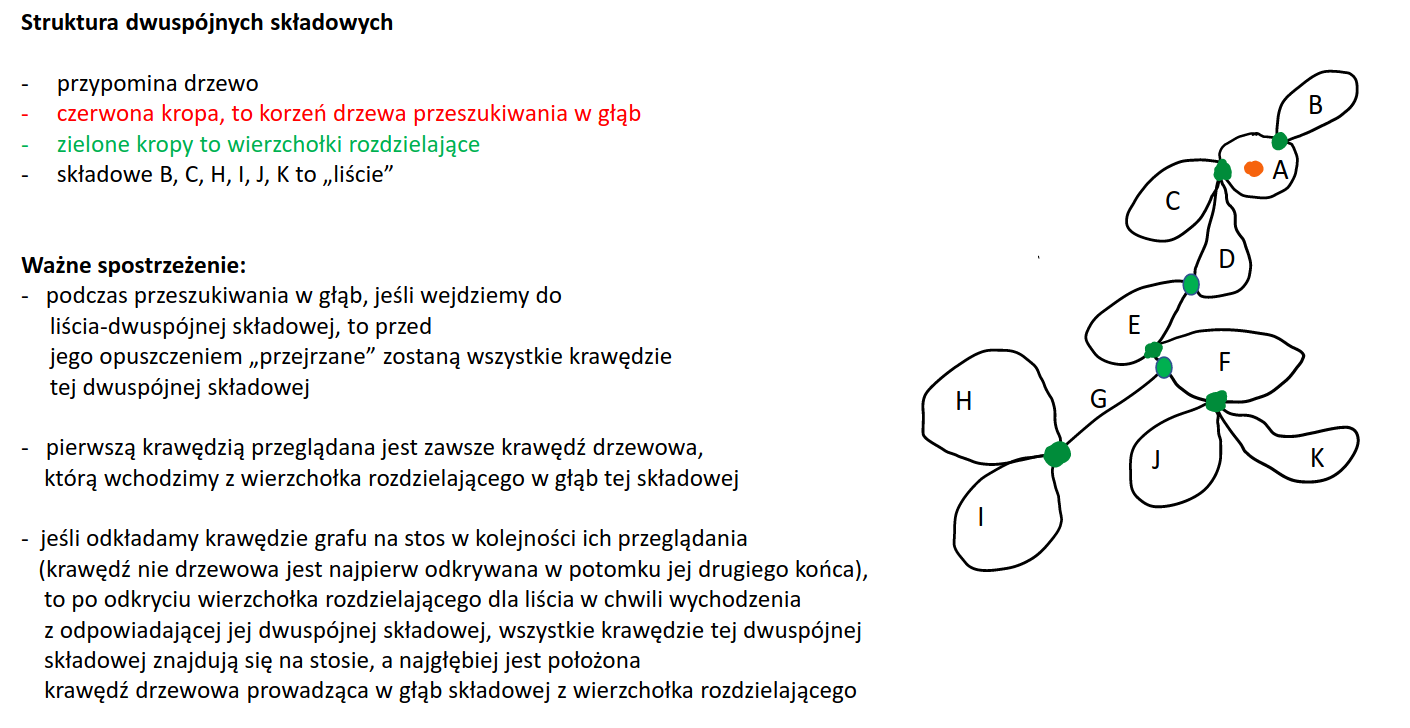
\includegraphics[scale=0.25]{sdwuspoj.png}

\entry
Istnieje algorytm znajdowania dwuspójnych składowych w czasie O(m)

